\documentclass[11pt,letterpaper]{article}
\usepackage[lmargin=1in,rmargin=1in,tmargin=1in,bmargin=1in]{geometry}
\usepackage{../style/homework}
\usepackage{../style/commands}
\setbool{quotetype}{true} % True: Side; False: Under
\setbool{hideans}{false} % Student: True; Instructor: False

% -------------------
% Content
% -------------------
\begin{document}

\homework{17: Due 11/28}{Great minds discuss ideas; average minds discuss events; small minds discuss people.}{Eleanor Roosevelt}

% Problem 1
\problem{10} Determine the mean value of the following: $-25$, $22$, $7$, $6$, $6$, $1$, $8$. \pspace

\sol The mean of the seven values $-25$, $22$, $7$, $6$, $6$, $1$, and $8$ is\dots
	\[
	\overline{x}= \dfrac{-25 + 22 + 7 + 6 + 6 + 1 + 8}{7}= \dfrac{25}{7} \approx 3.57143
	\]



\newpage



% Problem 2 
\problem{10} Consider the following numbers:
	\[
	27, \; 3, \; 33, \; 15, \; 47, \; 3, \; 22, \; 20, \; 9, \; 5
	\]
\begin{enumerate}[(a)]
\item Find the 5-number summary for the data.
\item Sketch a box plot of the data.
\item Find $P_{60}$. 
\end{enumerate} \pspace

\sol 
\begin{enumerate}[(a)]
\item Recall that the 5-number summary consists of the min, $Q_1$, median, $Q_3$, and the maximum. First, we order the data:
	\[
	3, \; 3, \; 5, \; 9, \; 15, \; 20, \; 22, \; 27, \; 33, \; 47
	\]
There are 10 numbers in this dataset. Therefore, the median is the average of the $\frac{10}{2}= 5$th and 6th numbers. Therefore, the median is $\frac{15 + 20}{2}= \frac{35}{2}= 17.5$. The first quartile, $Q_1$, is the median of the values less than the median: $3, 3, 5, 9, 15$. The median of these numbers is clearly 5 so that $Q_1= 5$. The third quartile, $Q_3$, is the median of the numbers greater than the median: $20, 22, 27, 33, 47$. The median of these numbers is clearly 27 so that $Q_3= 27$. The minimum of the original dataset is clearly 3 and the maximum of the original dataset is clearly 47. Therefore, the 5-number summary is\dots
	\[
	3, \qquad 5, \qquad 17.5, \qquad 27, \qquad 47
	\] \pspace

\item The interquartile range, IQR, for this dataset is $\text{IQR}= Q_3 - Q_1= 27 - 5= 22$. Then we have $1.5 \text{IQR}= 1.5 \cdot 22= 33$. But then we have $Q_1 - 1.5 \text{IQR}= 5 - 33= -28$ and $Q_3 + 1.5 \text{IQR}= 27 + 22= 49$. But then the box plot (using the convention that the whiskers extend to the threshold for an outlier) is\dots
	\[
	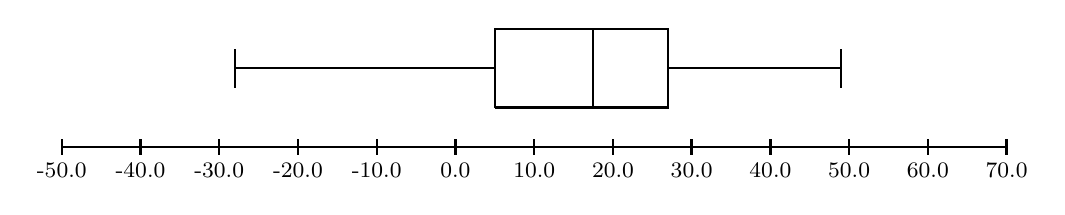
\begin{tikzpicture}
	\draw[line width=0.03cm] (0,0) -- (12,0);
	\foreach \x in {0,1,...,12} {
		\pgfmathsetmacro\tickval{-50 + 10*\x}
		\draw[line width=0.03cm] (\x,-0.1) -- (\x,0.1);
		\node at (\x,-0.3) {\footnotesize\tickval};
		}
	% Box
	\draw[line width=0.03cm] (5.5,0.5) -- (5.5,1.5) -- (7.7,1.5) -- (7.7,0.5) -- (5.5,0.5);
	% Midline
	\draw[line width=0.03cm] (6.75,0.5) -- (6.75,1.5);
	% Left Whisker
	\draw[line width=0.03cm] (2.2,1) -- (5.5,1);
	\draw[line width=0.03cm] (2.2,0.75) -- (2.2,1.25);
	% Right Whisker
	\draw[line width=0.03cm] (7.7,1) -- (9.9,1);
	\draw[line width=0.03cm] (9.9,0.75) -- (9.9,1.25);
	\end{tikzpicture}
	\] \pspace

\item There are 10 numbers in the dataset. But then $\frac{60}{100} \cdot 10= 0.6 \cdot 10= 6$. Then we know that $P_{60}$ is the average of the 6th and 7th number in the dataset. Therefore, $P_{60}= \frac{20 + 22}{2}= \frac{42}{2}= 21$. 
\end{enumerate}



\newpage



% Problem 3
\problem{10} Define what it means to be robust. Is the mean or median a robust measurement of `center'? Justify your response with an example. \pspace

\sol A measure is robust if it is `resistant' to outliers; that is, a measure is robust if the measures value does not `significantly' change if outliers are present (compared to when they are not). The mean is \textit{not} a robust measure of center, whereas the median is a robust measure of center. For instance, consider the dataset $\{ 1, 2, 3, 4 \}$. The mean and median for this dataset are 2.5. However, after adding the outlier 1,000,000 to this dataset, the mean is 200,002 while the median is 3. Observe that the addition of this outlier to the dataset greatly affected the mean but did not greatly affect the median. 


\end{document}